\documentclass[10pt,twocolumn,letterpaper]{article}

\usepackage{statcourse}
\usepackage{times}
\usepackage{epsfig}
\usepackage{graphicx}
\usepackage{amsmath}
\usepackage{amssymb}
\usepackage{booktabs}
\usepackage{tabularx}
\usepackage{hyperref}
\usepackage{wrapfig}


% Include other packages here, before hyperref.

% If you comment hyperref and then uncomment it, you should delete
% egpaper.aux before re-running latex.  (Or just hit 'q' on the first latex
% run, let it finish, and you should be clear).
\usepackage[breaklinks=true,bookmarks=false]{hyperref}
\usepackage{lipsum}
\usepackage{caption}
\usepackage{multicol}
\usepackage{kantlipsum}

\captionsetup[figure]{labelformat=empty}

\statcoursefinalcopy

% MARGINS
%-------------------------
%\usepackage[margin=0.8in]{geometry}
%-------------------------




\newcommand\myfigure[5]{%
  \ifdim#2>.8\linewidth
    {%
      \centering
      \includegraphics[width=#3]{#4}%
      \captionof{figure}{#5}%
    }%
  \else
  \begin{wrapfigure}{#1}{#2}
    \includegraphics[width=#3]{#4}
    \caption{#5}
  \end{wrapfigure}
  \fi
}







\setcounter{page}{1}
\begin{document}


%%%%%%%%%%%%%%%%%%%%%%%%%%%%%%%%%%%%%%%%%%%%%%%%%%%%%%%%%%%%%%%
% DO NOT EDIT ANYTHING ABOVE THIS LINE
% EXCEPT IF YOU LIKE TO USE ADDITIONAL PACKAGES
%%%%%%%%%%%%%%%%%%%%%%%%%%%%%%%%%%%%%%%%%%%%%%%%%%%%%%%%%%%%%%%



%%%%%%%%% TITLE
\title{Forecasting Stock Returns via Supervised Learning}

\author{Samuel Ilic\\
{\tt\small ilic@wisc.edu}
\and
Meenmo Kang\\
{\tt\small mkang84@wisc.edu}
\and
Jonathan Santoso\\
{\tt\small jsantoso2@wisc.edu}
}
% \setlength\parindent{0pt}
% \setlength{\parskip}{\baselineskip}%
% \setlength{\parindent}{0pt}%


% \makeatletter
% \renewcommand\paragraph{%
%     \@startsection{paragraph}{4}{0mm}%
%       {-\baselineskip}%
%       {.001\baselineskip}%
%       {\normalfont\normalsize\bfseries}}
% \makeatother
 

\maketitle
%\thispagestyle{empty}



% MAIN ARTICLE GOES BELOW
%%%%%%%%%%%%%%%%%%%%%%%%%%%%%%%%%%%%%%%%%%%%%%%%%%%%%%%%%%%%%%%


%%%%%%%%% ABSTRACT
\begin{abstract}
We incorporate the field of machine learning to study the age-old puzzle of forecasting time series stock returns. We implement a comparative analysis of various ensemble decision tree algorithms as well as an ordinary least squares regression for the purpose of out-of-sample return prediction. The ensemble methods implemented include Random Forest, Bagging and Boosting and are conducted within our analysis in an attempt to determine the best model. For simplicity, we focus on forecasting the returns of only a single stock, specifically IBM, using only OHLCV(open, high, low, close, volume) data from January 2002 to October 2018. Our implementation uses two different performance metrics to train our models, namely Mean Squared Error (MSE) and R-squared, in order to generate improved test set results. We find that the use of dimensionality reduction techniques, such as PCA and the LASSO, actually decrease the performance of our models. Lastly, we find that the boosted regression tree generalizes best to unseen data and has the best out-of-sample performance with a small but positive R-squared of 0.06\%. Thus, we have shown empirical evidence that the stock market is not completely efficient since one of the most highly liquid stocks, IBM, can be forecasted with some degree of accuracy.
\end{abstract}

%%%%%%%%% BODY TEXT
\section{Introduction}
Forecasting stock returns is an extraordinarily famous and notoriously difficult problem. When done successfully, proper implementation can generate billions of dollars. And, like the millions who have come before, speculation can get the best of anyone and an unsuccessful implementation could cost you your shirt. Making money in the stock market used to be about understanding companies from the ground up and valuing future cash flows. Using this methodology, investors and asset managers alike could only invest in at most a couple dozen companies. However, with the rise of technology and computational power, systematic investing began to take the spotlight and outperform the market. The focus of systematic investing is to combine statistics, computer science, and mathematics to isolate signals from noise to more accurately forecast returns by making high-frequency bets on a large basket of stocks. Still, many of the brightest minds have attempted to crack this enigma, but only a few have succeeded. The most famous of which being firms such as Renaissance Technologies, Two Sigma, and AQR Capital Management. Each of these firms has over a hundred PhDs and generates something on the order of two terabytes of daily data to make their forecasts. So how can a group of college students compete? Frankly, we cannot. However, we can simplify the problem by standing on the shoulders of giants through implementing proven methods and focusing only on a single stock. 

In our analysis, we implement four different supervised machine learning models with the goal of forecasting IBM's daily returns to generate a positive R-squared, more on this later. We specifically chose to use IBM due to the fact that it's a major corporation and a highly traded stock. What this means for our analysis is that IBM is efficiently priced and is one of the stock market's closest approximations to a random walk. Note that if IBM truly behaved like a random walk or a Brownian motion, any attempt at forecasting returns would be pointless. This follows from the simple reasoning that future returns should be theoretically independent of past returns. 

For each of our four models, we will optimize them across two different performance metrics, namely MSE and R-squared. The idea here is that MSE is the standard performance metric for regression and continuous forecasts. However, R-squared has been proposed within the financial community to be a more useful measure of performance when forecasting stock returns. As a result, both methods are implemented in order to see, empirically, which generalizes best on unseen data. 

With the benefit of hindsight, we know that certain stocks are easier to forecast than others. For example, Amazon's stock price has skyrocketed over the past 16 years, and as a result, even a linear model would generate positive predictive performance. However, for the purpose of investing, we have no idea ahead of time if Amazon or any other stock will go up down or sideways. In addition, IBM's price has shown a high degree of variability over our sample period which indicates that it's a very difficult stock to predict. For these reasons, we chose IBM because we will not fall into the trap tricking ourselves into thinking we build a predictive model by selecting an easy stock such as Amazon.

\section{Related Work}
Forecasting stock returns traditionally come in two basic forms. The first form is about predicting the difference in expected returns using a stock's fundamentals. Typically this is done via cross-sectional regressions and was popularized by Fama and French (1992). The second form focuses on forecasting time series regression returns using macroeconomic predictor variables. Note that these traditional methods have become rather antiquated and are no longer used in practice due to their inability to scale with increasing data. As a result, researchers have turned to machine learning in order to better handle the continuously increasing number of predictor variables. Machine learning has also been used to more efficiently and accurately price financial derivatives. However, the use of machine learning in forecasting stock returns, at least in academia, is relatively recent whereas hedge funds have likely been implementing it in secret for years. With respect to the use of decision trees in forecasting returns, Moritz and Zimmermann (2016) provide a great overview. In addition, there are other papers such a Gu, Kelly, and Xiu (2018) which provides a broad summary and comparative analysis of numerous machine learning methods. They find that regression trees and neural networks have the best out-of-sample predictive performance. This finding was the principal reason we decided to implement regression trees as opposed to an alternative method. They also propose that using R-squared rather than MSE is the new standard for accurately measuring and out-of-sample return prediction and training the model. Following the advice of Gu, Kelly, and Xiu (2018) we decided to begin our analysis using regression trees and were trained using R-squared as our measure of accuracy. With this in mind, our analysis varies significantly as we only focus on regression trees applied to a single stock whereas Gu, Kelly, and Xiu (2018) implement numerous machine learning algorithms to a portfolio of stocks on a much larger dataset going all the way back to 1960. 

\section{Proposed Method \& Experiments}
\paragraph{Clean Data \& Create Technical Indicator Variables} 
Any and all data used in our analysis was pulled directly from the Yahoo finance API via pandas-datareader in Python. As previously mentioned, we only gathered IBM data from January 1, 2002, to October 31, 2018. This is because, prior to 2002, the stock market had not yet converted to decimal prices and all stocks were priced in fractional increments of 1/16. This paved the way for high-frequency trading and sub-penny quoting of prices thus causing the market to behave radically different before and after 2002. Without getting into the weed's, the decimalization of stock prices made the market more efficient and led to tighter bid-ask spreads. Therefore, time series return forecasting models which use data prior to 2002 must account for the decimalization of prices or otherwise they risk optimistic bias in their results. For simplicity, we decided to ignore all data prior to 2002. 

Typically daily stock data from Yahoo finance is quoted in what is called OHLCV data. What this means is that our daily data came in the form as displayed in Table 1. The Date, Open, High, Low, and Close columns are all self-explanatory and relate to IBM's share price for the current day. Note that Volume indicates the total number of shares traded on any given day. This is an important column because it indicates how popular a stock it. Large spikes in trading volume can indicate that IBM's price is going to either fall or rise whereas low volume indicates that a stocks price will go sideways (price will remain stable). Lastly, the most important column is Adj Close. Often times, mature corporations such as IBM issue stock splits, stock buybacks, and dividends. Each of these actions can cause stocks price to decrease dramatically. For example, if IBM only has 100 shares and issues 100 new shares, then each share now becomes half as valuable and the stock price drops by a half. Thus, the Adjusted Close column takes these corporate actions into account and makes sure that the reported price only reflects trading activity. 


\begin{table}[h]
\resizebox{8cm}{!}{%
\begin{tabular}{llrrrrrr}
\toprule
Date &    High &     Low &    Open &   Close &   Volume &  Adj Close \\
\midrule
1/2/2002 &  121.50 &  119.80 &  120.60 &  121.50 &  6862800 &      84.68 \\
 1/3/2002 &  124.22 &  120.25 &  121.50 &  123.66 &  8621700 &      86.18 \\
1/4/2002 &  125.60 &  123.98 &  124.05 &  125.60 &  8405200 &      87.53 \\
1/7/2002 &  126.19 &  123.70 &  125.00 &  124.05 &  5939600 &      86.45 \\
1/8/2002 &  125.20 &  123.73 &  124.25 &  124.70 &  5311800 &      86.91 \\
\bottomrule
\end{tabular}}
\caption*{Figure 1: OHLCV Data from Yahoo Finance}
\end{table}

Since we are only concerned with the Adjusted Close prices, we dropped the Close price column. Then for simplicity of notation, we renamed the \textquoteleft Adjusted Close\textquoteright column to \textquoteleft Close\textquoteright. Recall that our analysis is concerned with forecasting stock returns and we do not yet have a returns column. Therefore, we calculated a daily returns as $\frac{\text{Adj Close}_t}{\text{Adj Close}_{t-1}}-1$ column named\textquoteleft Today\textquoteright using our newly named Close data according to the formula . We then created lagged return features for the past five days. This is a standard procedure in time series return forecasting as lagged returns are indicative of a stock's \textquoteleft momentum\textquoteright which is a market phenomenon and is a significant predictive variable. At this point, we began to consider technical indicators. A technical indicator is simply financial jargon for a new feature which was calculated on existing data. In other words, it's a mathematical calculation based on the historic price, daily return volume, or other information that aims to forecast the direction of a stock in the market. Technical indicators are often used by traders since they're designed to analyze short-term price movements. This means that many of them can become highly predictive under the right market conditions. However, they can be inappropriate for long-term analysis due to lack of enough information since they typically only focus on the last 2-3 weeks of data. We implemented 27 of the most popular indicators, which resulted in 27 newly created features. At the very end, we removed all row with missing values or NaN. 

\paragraph{Standardized Data and Create X \& y}
Prior to standardizing our data, we dropped all unnecessary daily data such as ‘High’, ‘Low’, ‘Open’, Volume’, and ‘Today’. This was done to eliminate the possibility of look-ahead bias. As its name implies, look-ahead bias means that your forecasting algorithm is using tomorrow's prices to determine today's trading signals. Or, more generally, it is using future information to make a ‘prediction’ at the current time. Obviously, this is not good and will artificially inflate a models performance and prediction accuracy. In addition, it's important to note that technical indicators come in two different forms, leading and lagging. Essentially, lagging technical indicators use past data to generate signals and are thus not prone to look-ahead bias. On the other hand, leading indicators use present data to generate signals and are prone to look-ahead bias. Therefore, to eliminate this bias, we shifted all lagging indicators back by one day. 

At this point, we have eliminated all possible look-ahead biases in our data and we begin to standardize our data. Note that our analysis focuses on regression trees and thus standardizing the data is not necessary. However, we chose to standardize our data for ease of comparison. In addition, we implement dimensionality reduction techniques such as PCA. Standardizing data before implementing PCA is important because the technique is all about maximizing variance and particularly for each component one at a time. This means that if our data is not standardized, features of different magnitudes can affect our PCs since each new axis is based on the standard deviation of the original variables. Our data was standardized via ‘StandardScaler’, one of the functions in Scikit-Learn. It is important to use the ‘StandardScaler’ function because at the end of our analysis we are able to take the inverse transform of our return forecasts. This allows us to make one-to-one comparisons between our forecasts and the realized returns. As for X and y, y is set to be the feature ‘Today’ (daily returns) and X includes all other variables.
\paragraph{Dimensionality Reduction}

Put simply, dimensionality reduction is the set of statistical techniques concerned with reducing the feature space of one's data. The main purpose of dimensionality reduction techniques is to avoid the curse of dimensionality and all the complexities associated with it. Often times, as in the case here, it is done to increase the performance of one's supervised machine learning model. There are many different algorithms and methods for dimensionality reduction but they all have the same basic focus. The idea of dimensionality reduction is to take a high dimensional dataset, which may have a number of collinear variables, and somehow remove all the unnecessary and uninformative columns/dimensions. Dimensionality reduction algorithms come in two different classes, both of which are explored in our analysis. The first class is called feature selection and the second class is called feature extraction. Note that we use both methods in our analysis in order to see if either can generate improved predictive performance over the original dataset. 

Feature selection is the more intuitive class and is concerned with selecting only the most important variables in the data. We implement the Least Absolute Shrinkage and Selection Operator (LASSO) in order to identify a sparse subset of predictors. Note that the LASSO is actually just a simple OLS regression with an added L1 penalty parameter. The benefit of the LASSO is that it bets on sparsity and can be used to select only the most important features in a dataset. This comes from the geometrical interpretation of an L1 norm being shaped like a diamond. Thus, when a LASSO regression is run on a high dimensional dataset, most parameter weights are directly set to zero. Even though LASSO is similar to an OLS regression, it does not have a closed form solution and it must be solved using a component-wise optimization algorithm such as the Shooting algorithm. In addition, the penalty parameter in the LASSO regression is actually a hyper-parameter and must be tuned. In our analysis, we tune our lambda coefficient (the LASSO penalty parameter) via 10-fold cross-validation. Recall that lambda of zero means that our LASSO regression is equivalent to an ordinary least squares regression. And, as we increase our lambda coefficient, we are actually increasing the sparsity of our solution such that the LASSO will select fewer significant variables.

Feature extraction is the second class of dimensionality reduction and it's concerned more with creating new features from old ones. The textbook example of feature extraction and the method implemented in our analysis is Principal Component Analysis (PCA). Hence, feature selection returns a subset of the original variables and feature extraction creates new variables by transforming the old data into a lower dimensional space. PCA works by using basic concepts from linear algebra such as eigenvalues and singular value decomposition. The goal of PCA is to explain away as much variation as possible in the original dataset by creating new features (Principal Components) which are simply orthogonal linear combinations of the original variables. PCA works at summarizing the original data into a lower dimensional space because it is able to simultaneously maximize variance (PCs are orthogonal) and reconstruct the original data set (PCs are linear combinations of original variables). The last major aspect of PCA, after constructing all the principal components (PCs), is to select the number of features to retain. The easiest and most common method for retaining PCs is to implement a scree plot and look for the elbow. The idea here is that the elbow in signifies the point at which any additional variables provides decreasing marginal benefit. However, I feel that this method is not grounded in mathematics. I favor an alternative method of utilizing the PCAs computed eigenvalues to determine the total number of PCs to retain. If a PC has a variance greater than 1, then this implies that it is associated eigenvalue must also be greater than 1. Intuitively, what this means is that a PC with an eigenvalue greater than 1 actually explains more variance in the data than any of the original features. We retain all the principal components with eigenvalues greater than 1.

One major downside of PCA and LASSO exists which comes up in our forecasting step. Specifically, when predictors are highly correlated, both PCA and LASSO can lead to suboptimal forecasts. For time series forecasting under highly correlated data, such as our technical indicators, the LASSO is often inferior to taking an average of the predictors and using it as the sole predictor. This is the case if say all of the predictors are equal to the target function plus some white noise. PCA works better than the LASSO, in our case because it's concerned with forming a linear combination of the predictors to isolate the signal by reducing noise. However, the drawback of PCA is that in the dimension reduction step it doesn't incorporate our ultimate objective of forecasting returns. Hence, it condenses our data prior to the forecasting step and pays no considerations to how the predictors are associated with future returns. 

\paragraph{Model Selection: Decision Trees \& Multivariate Regression}
Decision trees are a form of supervised machine learning algorithms which employ an if-then-else decision methodology to fit data and forecast results. Inherently, decision tree algorithms employ a greedy search, based on the feature set, in order to maximize the information gain or minimize entropy at each split. However, for regression trees, as in the case of our analysis, the algorithm employs recursive binary splittings to minimize the residual sum of squares (RSS). As a result of the greedy search process, decision trees make locally optimal decisions and will forecast the same results when the model is fitted on identical data. The regression tree algorithm works naturally for the purpose of predicting stock returns due to its stability with continuous values.  Moreover, some of the advantages of the regression tree algorithm include simplicity of interpretation, little feature preprocessing, and logarithmic prediction complexity. Often times, regression trees tend to be unstable and overfit the data. To combat this problem we implemented pre-pruning. We chose not to implement the method of post-pruning as it's known for being technically difficult and was not discussed sufficiently in class. 

In addition to pruning one's regression tree, another method for improving the predictive performance is to fit many separate trees and combine them into a statistical ensemble. The Random Forest, Bagging, and AdaBoost algorithms represent some of the most popular ensemble methods and are just extensions of the regression decision trees algorithm. Bagging works by implementing the bootstrap algorithm to combat the natural tendency of a decision tree to be a high-variance estimator. It works by combining many different regression trees, each of which being fit on separate bootstrap samples. For the purpose of time complexity, we implemented the bagging algorithm such that it only selected the square root of the total number of features, for each iteration. However, a major complication associated with Bagging is that many of the fitted regression trees are highly correlated. To combat this problem, the Random Forest algorithm is essentially identical to Bagging with the exception that it makes use of feature bagging. The difference is that feature bagging randomly selects a subset of features at each split. In our implementation, we again chose to randomly select the square root of the total number of features. This sounds counterintuitive but it actually serves to decrease the variance of the final model by decreasing the correlation between each successive tree. 
The Scikit-Learn implementation of both the Bagging and Random Forest algorithms include the parameters' maximum depth and minimum sample split. We used both of these parameters in order to pre-prune our ensemble models and prevent overfitting. The Bagging regressor algorithm is very similar to the Random Forest algorithm in that it utilizes bagging, or sub-sampling of the dataset, in order to prevent overfitting. In our project, we utilized decision tree regressor as the base estimator which is the default in the Scikit-Learn implementation. With respect to Boosting, the AdaBoost regressor also utilizing a decision trees its base estimator. Boosting is another variation of the regression tree where the algorithm iteratively fits weak learners which are adjusted in order to favor misclassified points made by the previous learner. This classifier is known as an  \textquoteleft out of the box\textquoteright algorithm and is usually considered one of the best predictive models before the prevalence of neural networks. 

Lastly, we have Multivariate Linear Regression which was implemented in our analysis to serve as the benchmark model. Multivariate Linear Regression is a supervised machine learning algorithm that calculates weights on all the features in order to generate a prediction. It's fitted utilizing the least squares principle to minimize loss (the residual sum of squares). This algorithm is one of the simplest as it has a closed form solution. The downside to Multivariate Linear Regression is that it works under the assumptions of homoskedasticity, linearity, independence of errors, lack of multicollinearity, and weak exogeneity. 

Each of these algorithms was chosen as part of the project primarily due to their simplicity and ability to predict continuous values. In addition, due to the minimal assumptions needed for the regression tree algorithms, these models were appropriate for the project. With limited computing power, each of these algorithms could run in a reasonable amount of time even with a large number of estimators.

\paragraph{Performance Evaluation: R-Squared,  MSE & Historical Mean Returns}
One of the most common performance evaluation metrics used in forecasting returns is to compare predictions against Historical Mean Returns. This metric makes sense in many financial applications but in the case of analyzing a single stock, it's flawed. It seems sensible to have one's forecasts be as close as possible to the Mean of the Historical Returns. However, it's been shown that this form of performance evaluation almost always leads to significant underperformance of a naive zero forecast. Intuitively, this makes sense because historical mean returns are actually very noisy. This means that if we training our model on Historical Mean Returns, we will actually be implicitly lowering the bar for good performance. 

Since MSE is the hallmark of continuous performance evaluation, it's no surprise that we use it to train our decision tree models. However, there's one aspect of MSE that makes it subpar for the purpose of return prediction. That is, what' the benchmark and at what point does an MSE turn from good to bad? There's no intuitive answer to this question. As a result, we turn our attention toward an alternative metric for performance evaluation and use R-squared. The use of R-squared solves both of the issues brought up of Historical Mean Returns and MSE. Specifically, by benchmarking our R-squared to a value of zero we don't artificially inflate our performance and we have an intuitive sense of the model's predictive power. This is an important choice because as pointed out by Gu, Kelly, and Xiu (2018), benchmarking our model against Historical Mean Returns will artificially inflate our R-squared by roughly 3\%. On another note, Gu, Kelly, and Xiu (2018) state that their out-of-sample R-squared using decision trees was 0.27\%. In addition, it's often noted that an R-squared between 0.20\%-0.25\% in large enough to start your own hedge fund (depending on the specific strategy). We make a note of pointing this out to indicate how difficult it is to forecast stock returns and generate any form of predictive power. These metric set the baseline for what we consider to be a successful project. Any model with a positive R-squared is considered to be a success.

\paragraph{Time Series Train-Test Splits}
In order to avoid look-ahead bias (data leakage) while training our models, we can't implement the standard cross-validation techniques, as presented in class. This is because data leakage is an especially tricky issue when it comes to time series as financial data is serially correlated. We mentioned this issue earlier when discussing the creation of our X & y datasets. It would be a mistake to implement cross-validation to produce training and test sets as it randomly splits the data. This leads to making erroneous errors in our forecasts as we would essentially be making predictions about, say, 2014 while using data from 2015. This is an issue because if we are making predictions about 2014, data from 2015 should be unavailable. To solve this issue, we implemented TimeSeriesSplit as displayed in Figure 2. 

TimeSeriesSplit was used for both parameters tuning as well as forecasting returns. But first, we split our data, X & y, into training-validation and test sets. This split was chosen to be the beginning of 2018. This was done for the purpose of imagining we are at the end of 2017 and was want to train a model to forecast returns for 2018. Hence, our training-validation set included data from 01/01/2002 - 12/31/2017 & our test set included data from 01/01/2018 - 10/31/2018. Within the training-validation set, we used TimeSeriesSplit to train our model. Then, in our test set, we again used TimeSeriesSplit to test our model's performance. This was done under the idea that we wanted to use the most up-to-date model which was trained on all available data to make our predictions. For example, if we are forecasting returns for October 2018 it would make sense to use the best model which was trained on all available data rather than one which was only trained using data prior to 2018. The use of TimeSeriesSplit means that our training and test set performance is directly related to our chosen number of train/test splits. Hence, the larger our train/test splits, we are able to train more models on more data and obtain increase out-of-sample performance. However, the downside to increasing the number of train/test splits is the increasing time complexity of the model. As a result, we settled at using only 10 train/test splits for both our train-validation and test sets. 

\begin{figure}[h]
  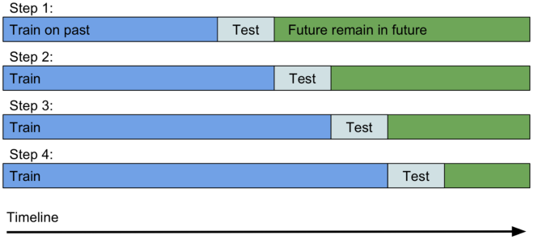
\includegraphics[height=2.5cm, width=8.5cm]{Plots/Figure2.png}
  \caption{Figure 2: TimeSeriesSplit for both Hyper-parameter Tuning and Forecasting}
\end{figure}

\paragraph{Parameter Tuning}
Recall that the models we are implementing include Random Forest, Bagging, Boosting, and Linear Regression. We chose to implement four different models for the purpose of our analysis to determine which, if any, can generate positive predictive performance. To make the parameter tuning process as simple as possible, we created wrapper functions for each model such that it would also execute TimeSeriesSplit. We set the parameters of each wrapper function to determine both the hyper-parameters of each model as well as the number of train-validation splits which will be executed in the TimeSeriesSplit. At the beginning of each wrapper function, we would initialize an empty list to for our computed R-squared and MSE values. We would then divide the total training set into train-validation splits and loop through each one. Each model would be fitted on the training set and would be tested/make predictions on the validation set.

In order to fit the best model, our objective was to obtain the largest R-squared as well as the smallest MSE. We believe the most important choice in optimizing our models came from how we settled on the best R-squared and MSE's. Note that if we simply selected the model with the largest R-squared on the final validation set, then our model has likely overfitted our data and it will not generalize well on the test set. To combat this issue, we decided that the best model was the one the one with the largest average R-squared and the smallest average MSE across all the validation sets. Hence, we would select the model with the best average performance across the entire validation set. We believed that this model would generalize to unseen data and have the best out-of-sample forecasts. At this point, we were still uncertain to whether R-squared or MSE was the best performance evaluation metric. So, we decided to optimize each model separately according to both. 

Perhaps the most important hyper-parameter for each ensemble technique is the total number of estimators. This was the first hyper-parameter we tuned was done on the base decision tree model with all default settings and can be seen in Figure 3. We determined that the optimal number of estimators for each ensemble method was 150. At this point and increase in the number of estimators only leads to marginal increases in performance but leads to increased computational complexity. For all other parameters in each model, we applied a grid search. The hyper-parameters we chose to evaluate were the minimum number of samples required to split a node, the max depth of the decision tree, the maximum number of features to consider for each split and the learning rate for a boosting.

\begin{figure}
  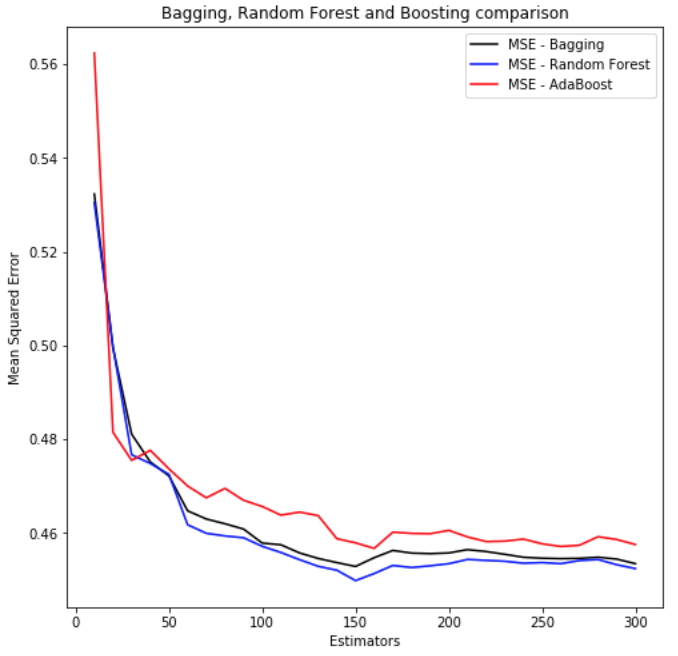
\includegraphics[height=5.5cm, width=6.5cm]{Plots/Comparison.png}
  \caption*{Figure 3: Selecting the Total Number of Estimators for each Ensemble Method}
\end{figure}

\paragraph{Software}
\begin{itemize}
    \item Python
    \begin{itemize}
        \item ML: Scikit-Learn, MLxtend
        \item Visualization: Matplotlib, Seaborn
        \item Others: SciPy, NumPy, Pandas
    \end{itemize}
    
    \item Primary Working Environment
\begin{multicols}{2}
\begin{itemize}
\item Jupyter
\item Anaconda

\end{itemize}
\end{multicols}
    
    \item GitHub\\ \url{ https://github.com/meenmo/Forecasting_Stock_Returns_via_Supervised_Learning}
\end{itemize}

\section{Results \& Discussion}

% \begin{figure}[htb]
%     \caption{Figure 4: Optimal Hyper-parameters for Each Algorithm}
%     \begin{minipage}[t]{.2\textwidth}
%         %\centering
%         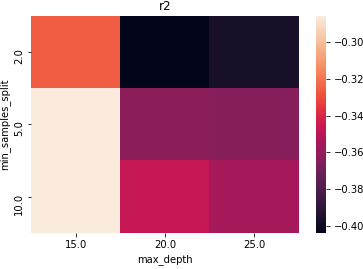
\includegraphics[width=\textwidth]{Plots/Best_Model_RF.png}
%     \end{minipage}
%     \begin{minipage}[t]{.2\textwidth}
%         %\centering
%         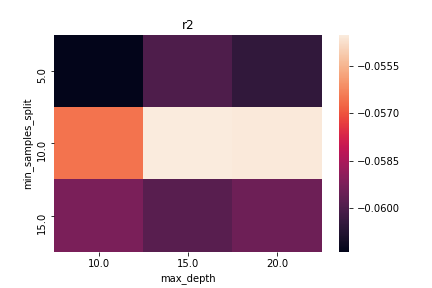
\includegraphics[width=\textwidth]{Plots/Best_Model_Bagging.png}
%     \end{minipage}
%     \hfill
%     \begin{minipage}[t]{.2\textwidth}
%         \centering
%         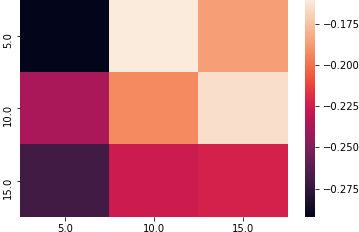
\includegraphics[width=\textwidth]{Plots/Best_Model_Boosting_2.png}
%     \end{minipage}  
%     \label{fig:1-2-3}
% \end{figure}


\myfigure{L}{.5\linewidth}{\linewidth}{Plots/Best_Model_RF.png}{}

Through utilizing a 10 fold TimeSeriesSplit and storing the resulting predictions on the validation set, we were able to obtain our baseline MSE and R-squared values. Note that these baseline values were computed by taking the average MSE & R-squared values across all 10 TimeSeriesSplits. In order to improve upon our baseline models, we conducted hyperparameter tuning on the minimum samples split and the maximum depth parameters. The heat map in Figure 4 depicts the optimal hyperparameters for each of our ensemble algorithms on the validation set. It can be observed, in general, that as the maximum depth of the decision tree increases and as minimum sample leaf decreases, the algorithms will tend to overfit. This results in an optimistic training-validation set performance and decreased generalization performance on the test set. Thus, in order to obtain the best performing model, we need to determine both the optimal tree depth as well as the minimum sample leaves at the same time. With respect to Adaboost, we also chose to vary the learning rate to penalize our model against overfitting. For Linear Regression, there are no hyperparameters to optimize as there exists a closed form solution.


\begin{table}[h]
\resizebox{8cm}{!}{%
\begin{tabular}{llrrrrrr}
\toprule
&    Random Forest &    Bagging &   AdaBoost (with rate 1.0) \\
\midrule
Max Depth &  15 &  15 &  5 \\
Min Sample Split &  10 &  10 &  5 \\
\bottomrule
\end{tabular}}
\caption*{Figure 5: Optimal Hyper-parametersof Each Model}
\end{table}

After hyperparameter tuning, we were able to obtain the parameters for our final model. These can be seen in the table above. Recall that after obtaining our final models we again ran a 10 fold TimeSeriesSplit on our test dataset in order to train our model and make forecasts. The results of our final models are summarized in Figure 6. This table indicates that all of our models produced a negative R-squared with the exception of Boosting. Note that this table only shows the models which were trained via maximizing R-squared. This is because optimizing with respect to R-squared lead to significant outperformance as opposed to optimizing with respect to MSE. Recall that a negative R-squared indicates that our model actually performs worse than the trivial model which forecasts zero every time. Hence, our Boosting model is the only one which outperforms a horizontal line! Our benchmark Multivariate Linear Regression model actually performed the worst. This is likely due to underfitting of the data as stock returns are highly complex and clearly aren't linear. However, our Adaboost algorithm has a positive R-squared of 0.06\%. Note that even a positive R-squared value is a very difficult feat to accomplish due to the random nature of the stock market and its close approximation to a Brownian motion. We find that our  0.06\% R-squared is highly significant as it was obtained using nearly all of IBM's 2018 returns. 


\begin{table}[h]
\resizebox{8cm}{!}{%
\begin{tabular}{llrrrrrr}
\toprule
&    Random Forest &    Bagging &   Boosting & Linear Regression \\
\midrule
$R^2$ &-0.100561&-0.0414371&0.00634&-0.26312\\
MSE &1.17259&1.1096&1.05866&1.34579 \\
\bottomrule
\end{tabular}}
\caption*{Figure 6: Final Predictions}
\end{table}

Universally, across all our models, we observed that the most significant predictive variable was Moving Average Convergence Divergence (MACD). Coincidentally, this happens to be one of the most popular technical indicators used in practice. Put simple, MACD is a simple trend following momentum indicator which shows the relationship between two different moving averages on IBM's price. It essentially serves as a signal to indicate when a price has risen/dropped by too much and will correct back to its 26-day moving average. This indicator helps an investor understand whether stock prices are strengthening or weakening which results in a strong correlation with future stock returns. In addition, another strongly predictive feature was the 14-day Exponential Moving Average (EMA). Essentially, an EMA is just a moving average of a stock's returns where the last few days are given larger weights. 

\begin{figure*}
  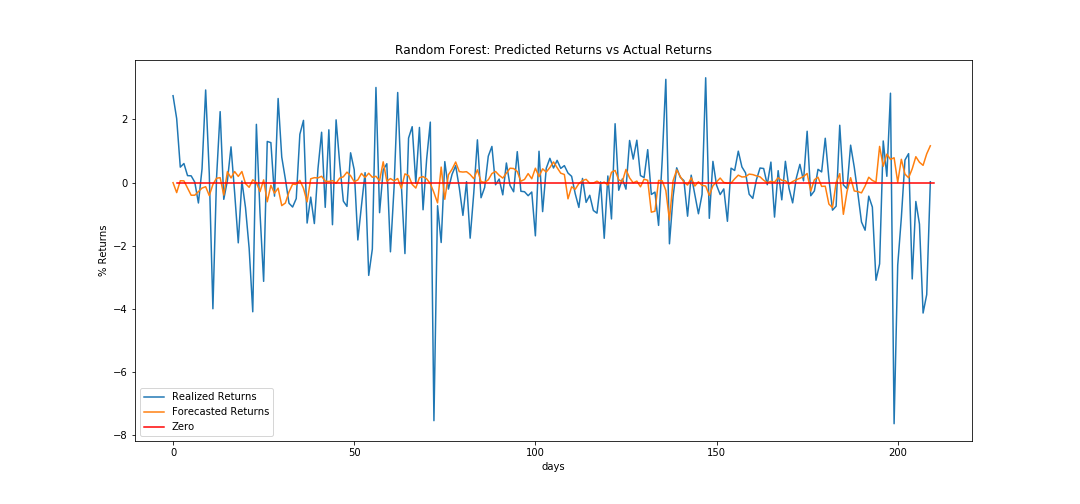
\includegraphics[width=\textwidth,height=6cm]{Plots/RF_Predicted_Returns_Actual_Returns.png}
  \caption{Figure 7: Forecasted Returns with Boosting}
\end{figure*}


In addition to forecasting returns, we also wanted to get a sense for how our models forecasted the direction of the stock price. Hence, even though our main interest is in forecasting the magnitude of the returns, we wanted to understand why most of our models obtained negative R-squared values. We postulated that it may be due to incorrectly forecasting the direction of the returns. As a result, we revised our models to only forecast the direction of the future returns. Our binary prediction was set such that zero indicated a negative return and a one indicated a positive return.  The result of our binary classification process is illustrated in the confusion matrices of Figure 8. We observe that our Random Forest model had the best binary classification accuracy even though it had a negative R-squared. This is an interesting result as our Random Forest model actually had the worst R-squared performance, even compared to the linear model. Another impressive finding is that all four of our models have over 50\% classification accuracy. 
\begin{figure}[h]
  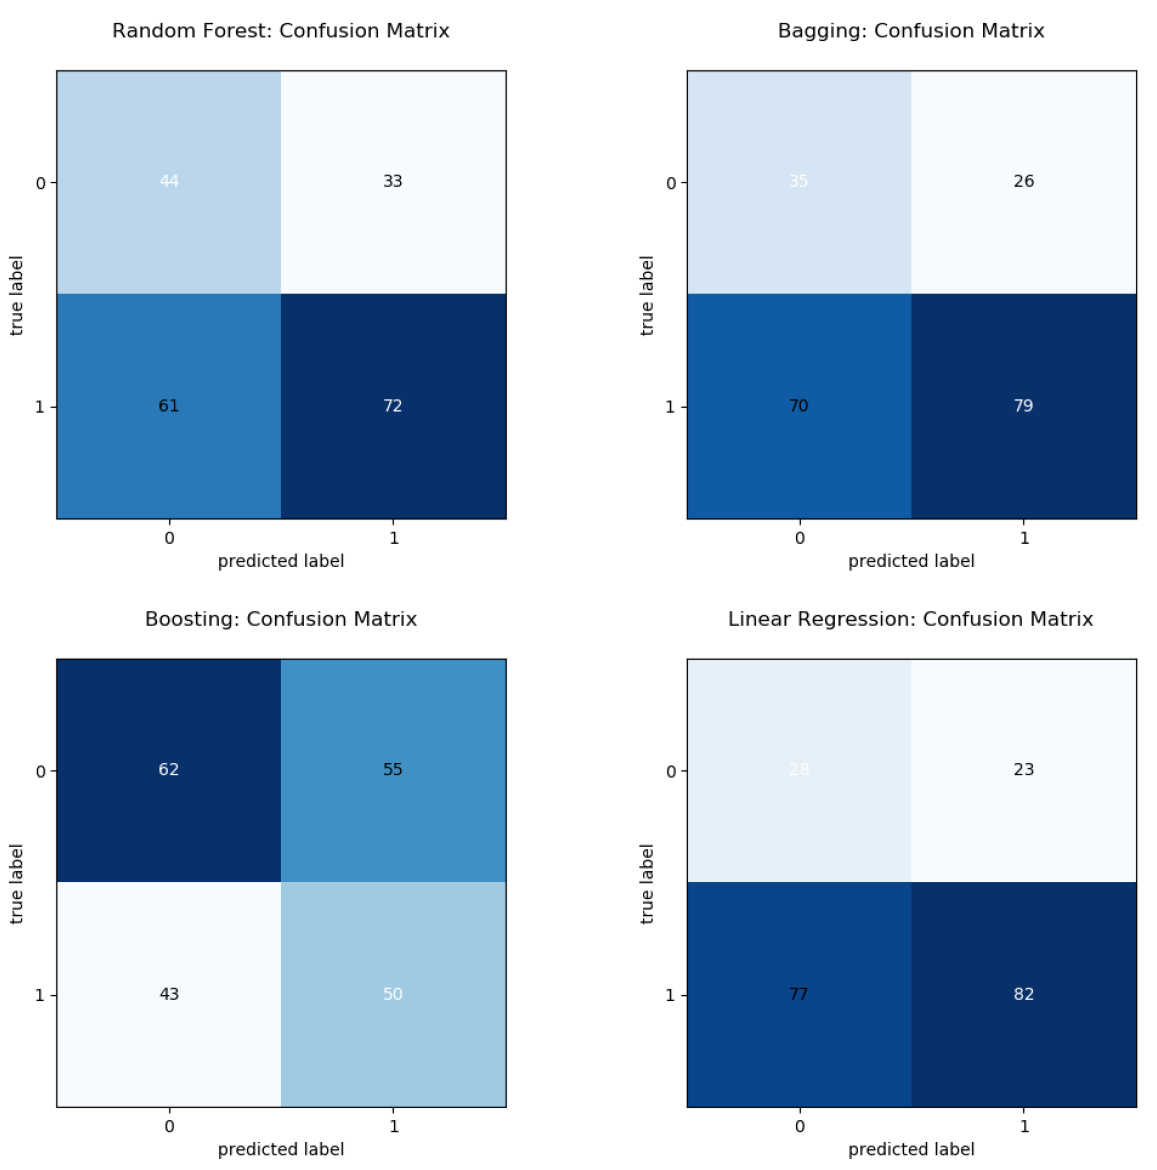
\includegraphics[height=7.5cm, width=7.5cm]{Plots/ConfusionMatrix.png}
  \caption{Figure 8: Confusion Matrices for Binary Prediction}
\end{figure}

\begin{table}[h]
\resizebox{8cm}{!}{%
\begin{tabular}{llrrrrrr}
\toprule
&    Random Forest &    Bagging &   Boosting & Linear Regression \\
\midrule
Accuracy &55.23\% &54.29\% &53.33\% &52.38\%\\

\bottomrule
\end{tabular}}
\caption*{Figure 9: Binary Prediction Accuracy}
\end{table}
This indicates that we were, on average, correctly forecasting the direction of IBM's returns. However, this does not explain the negative R-squared values from nearly all of our models. One would imagine that correctly forecasting the direction of stock returns would at least result in a positive R-squared value. However, this clearly was not the case with our models. In addition, we can see that our Boosting model only outperformed the linear model with respect to classification but had the largest R-squared value. This suggests that the major issue in our forecasting models was not that we were not correctly forecasting the direction but that we were incorrectly forecasting the magnitude of the returns. Specifically, our negative R-squared values are likely the result of our model's forecasting, on average, large returns. Hence, our R-squared values would take a large hit each time our model forecasted a large return which differed in direction of the realized return. Accessing this intuition further, we can see that in Figure 7 our Boosting algorithm, on average, had very small forecasted returns which were often only a fraction of the size of the realized return.

Going Further, we applied the min-max scaler form sklearn in order to obtain binary probabilities for our stock return forecasts. Based on these probabilities, a ROC plot was generated and is shown in Figure 10. Using area under the the ROC curve as the metric, we now find hat Bagging had the best classification performance. It's hard to determine the specific reason behind why bagging produced the best ROC AUC, due to the complexity of stock data and the negligible difference each AUC we obtained (The difference between the accuracy of bagging and boosting is only 0.003\%). Anyhow, all four of our models performed better than random, or 50\%, which is a satisfactory result considering how difficult it can be to forecasts stock returns.

Further, min/max scaler from sklearn was employed to obtain binary probabilities of stock returns whether it goes up or down. Based on these probabilities, the ROC plot was generated below and we calculated the best algorithm identifying those whose area under the curve is the biggest; Hence, bagging turns out to be the best performing algorithm for this implementation. It is hard to determine specific reason why bagging produced the best figure in ROC due to the complexity of stock data and negligible difference each AUC we obtained (The difference between the accuracy of bagging and boosting is only 0.003\%.). Anyhow, all four algorithms produced better prediction than random, or 50\%, which is satisfactory results considering the fact that randomness of stock price. We also made sure that all the testing set have balanced 0 and 1. 

\begin{figure}[h]
  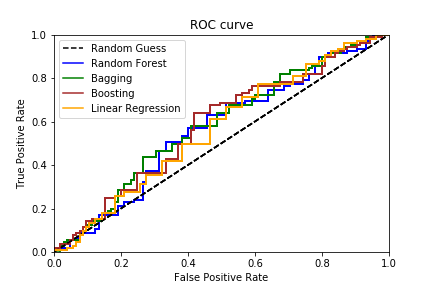
\includegraphics[height=6cm, width=8cm]{Plots/ROC_Curve_1.png}
  \caption{Figure 10: ROC Curve}
\end{figure}

\begin{table}[h]
\resizebox{8cm}{!}{%
\begin{tabular}{llrrrrrr}
\toprule
&    Random Forest &    Bagging &   Boosting & Linear Regression \\
\midrule
Accuracy &0.552\%&0.571\%&0.568\%&0.549\%\\
\bottomrule
\end{tabular}}
\caption*{Figure 11: Area Under Curve}
\end{table}



\section{Conclusion}
In this paper, we implemented a comparative analysis of Bagging, Random Forest, Boosting, and Multivariate Linear Regression in order to determine the best model for the purpose of forecasting IBM's daily stock returns. At the highest level, we find that all of our ensemble methods add significant predictive performance over a simple multivariate linear regression. In addition, we find that standard dimensionality reduction techniques such as PCA and LASSO reduce the out-of-sample performance across all our ensemble methods. This is likely due to the fact that both methods reduce the dimensionality of the original dataset prior to forecasting and thus pay no consideration to how the predictors are associated with future returns. We could improve upon this issue in further analysis by using an alternative dimensionality reduction technique such as Partial Least Squares which explicitly accounts for covariance between the predictor variables and the variable which is being forecasted. We also find that tuning our supervised learning models according to R-squared led to improved predictive performance over tuning via MSE. Lastly, our Boosting regression tree had the best out-of-sample predictive performance with a positive R-squared of .06\% whereas all other models had a negative R-squared. Our positive predictive performance indicates IBM's stock is not efficient and does not reflect all publicly available information. 

There are many ways in which our project could have been improved. For further analysis, one could improve the breadth of the dataset beyond technical indicators to also include other significant financial factors. In addition, we only explored the process of pre-pruning, however, a more sophisticated post-pruning method such as cost-complexity pruning could also be employed. And lastly, the implementation of an alternative dimensionality reduction technique such as Partial Least Squares has the potential to significantly improve our predictive performance as well as decrease computational complexity. 

\section{Contributions}
{\bf Samuel Ilic (Supreme Leader)}: Analyzed and gave financial background to all team members. Was involved in coordination and managing the project and also lead data collection and cleaning. In addition, Sam focused on dimensionality reduction, training & tuning of all models, interpreting results, organizing the presentation, and writing the final report.

{\bf Meenmo Kang (Data Wizard)}: was primarily responsible for data cleaning and data visualization. Meenmo also focused on initial analysis to identify potential outlier points and exclude them from our analysis. Further feature engineering from base dataset was done by Meenmo and Jonathan.

{\bf Jonathan Santoso (Model Ninja)}: Created lagged stock return features, helped out in the selection of machine learning algorithm, and hyper-parameter tuning via grid-search. Moreover, Jonathan was involved in determining cross-validation splits and also helped out with the interpretation of results.



\newpage
\onecolumn
\section{Work Cited}
\begin{enumerate}
    \item Fama and French (1992) - The Cross-Section of Expected Stock Returns
    
    \item Moritz and Zimmermann (2016) - Tree-Based Conditional Portfolio Sorts: The Relation between Past and Future Stock Returns
    
    \item Gu, Kelly, and Xiu (2018) - Empirical Asset Pricing via Machine Learning
    
    \item Peter Bakker (2018) - Technical analysis Indicators without Talib\\ \url{https://www.quantopian.com/posts/technical-analysis-indicators-without-talib-code}

    \item Pandas Technical Indicators: Technical indicators.py \url{https://github.com/Crypto-toolbox/pandas-technical-indicators/blob/master/technical_indicators.py}
    
    \item Visualizing cross-validation behavior in Scikit-learn\\  \url{https://scikit-learn.org/stable/auto_examples/model_selection/plot_cv_indices.html#sphx-glr-auto-examples-model-selection-plot-cv-indices-py}
    
    \item TimeSeriesSplit\\  \url{https://scikit-learn.org/stable/modules/generated/sklearn.model_selection.TimeSeriesSplit.html}
    
    \item Yahoo Finance -  \url{https://finance.yahoo.com/quote/IBM}
    
    \item Investopedia \\  \url{https://www.investopedia.com/terms/d/decimal-trading.asp}
    
    \item Technical Indicators \\ \url{https://www.investopedia.com/terms/t/technicalindicator.asp}
    
    \item Avoiding Data Leakage \\  \url{https://conlan.io/blog/data-science/avoiding-data-leakage-machine-learning/}
    
    \item Python - Python Software Foundation. Python Language Reference, version 3.6. Available at  \url{http://www.python.org}
    
    \item Scikit-Learn - Scikit-learn: Machine Learning in Python, Pedregosa et al., JMLR 12, pp. 2825-2830, 2011
    
    \item SciPy - Jones E, Oliphant E, Peterson P, et al. SciPy: Open Source Scientific Tools for Python, 2001-, \url{http://www.scipy.org/}
    
    \item Pandas - Wes McKinney. Data Structures for Statistical Computing in Python, Proceedings of the 9th Python in Science Conference, 51-56 (2010) (publisher link)
    
    \item NumPy - Travis E, Oliphant. A guide to NumPy, USA: Trelgol Publishing, (2006).
    
    \item Matplotlib - John D. Hunter. Matplotlib: A 2D Graphics Environment, Computing in Science & Engineering, 9, 90-95 (2007), DOI:10.1109/MCSE.2007.55 (publisher link)
    
    \item MLxtend - Raschka, Sebastian (2018) MLxtend: Providing machine learning and data science utilities and extensions to Python's scientific computing stack. J Open Source Softw 3(24).
    
    \item TimeSeriesSplit Picture \\ \url{https://medium.com/cindicator/backtesting-time-series-models-weekend-of-a-data-scientist-92079cc2c540} 
    
    \item How To Backtest Machine Learning Models for Time Series Forecasting \\
    \url{https://machinelearningmastery.com/backtest-machine-learning-models-time-series-forecasting/}
\end{enumerate}



% {\small
% \bibliographystyle{ieee}
% \bibliography{bibliography.bib}
% }

\end{document}
